\section{Matrix multiplication}
\lecture{6}{11/11}

\begin{algorithm}
    Naive matrix multiplication
    It is clear that we can construct a simple naive algorithm to calculate the product of two matrices using the formula
    \[ c_{ij} = \sum_{k = 1}^{q} a_{ik}b_{kj}. \]
\end{algorithm}

In this naive algorithm, 
it is clear that we have $p \cdot r \cdot q$ scalar multiplications 
(look at the formula above).

We know that matrix multiplication is associative, 
that is for compatible matrices $A_1, A_2, A_3$ we have
\[ A_1(A_2 A_3) = (A_1A_2)A_3; \]
however, running both of these on our naive algorithm can have quite a large difference in running time. 
Let's illustrate this.

\begin{example}[Matrix multiplication running time]
    Let $A_1 \in M_{10 \times 100}(\R)$, $A_2 \in M_{100 \times 5}(\R)$, $A_3 \in M_{5 \times 50}(\R)$. $(A_1A_2)A_3$ involves calculating $A_1A_2$ then $(A_1A_2)A_3$, so we have
    \[ (10 \times 100 \times 5) + (10 \times 5 \times 50) = 7500. \]
    Alternatively, if we calculate $A_1(A_2A_3)$ we get
    \[ (100 \times 5 \times 50) + (100 \times 50 \times 10) = 75000. \]
\end{example}

\begin{problem}
    Let $(A_1, A_2, \ldots, A_n)$ be $n$ compatible matrices and we wish to calculate $A_1 \cdot A_2 \cdot \ldots \cdot A_n$. 
    So we have $A_i \in M_{p_{i - 1} \times p_i}$ for some sequence $p_i$. 
    Where should parantheses be placed so as to minimise the number of operations to calculate the product?
\end{problem}

Let's investigate the running time of a brute force solution to this problem. 
Let $P(n)$ denote the number of ways to parenthesise a product of $n$ matrices ($n \geq 2$). 
We have $P(2) = 1, P(3) = 2, P(4) = 5, \ldots, P(n) = C_{n - 1}$ 
where $C_n$ is the $n$th \emph{Catalan number}. 
We have that
\[ C_n = \frac1{n + 1} \binom{2n}{n} \sim \frac{4^n}{\sqrt{\pi} n^{\frac3n}};  \]
hence, 
a brute force algorithm will have exponential running time. 
Obviously, this is not very good. 
Let's look at applying dynamic programming.

We denote $A_{i..j} = A_i \cdot A_{i + 1} \cdot \ldots \cdot A_j$ for $i \leq j$. 
To paranethesise $A_{i..j}$, 
we must split between two matrices $A_k$ and $A_{k + 1}$, $i \leq k < j$ and it 
must be optimal.

We let $m(i, j)$ denote the minimum number of multiplication to calculate $A_{i..j}$. 
Then
\[ m(i, j) = \min_{i \leq k < j} \{ m(i, k) + m(k + 1, j) + p_{i - 1}p_kp_j \}. \]
For explanation, 
the $m(i, k)$ is the minimum number of multiplications before the split, 
$m(k + 1, j)$ is the minimum number of multiplications after the split, 
and $p_{i - 1}p_kp_j$ 
is the number of multiplications to combine the two matrices in the split. 
We of course have $m[i, i] = 0$.

So now we build our solution. 
Our inputs will be the sequence $(p_n) = (p_1, p_2, \ldots, p_n)$ 
for the matrices $A_1, A_2, \ldots, A_n$ such that $A_i \in M_{p_{i - 1} \times p_i}(\R)$. 
From this, we construct the following algorithm.

\begin{algorithm}
    Bottom-up dynamic programming for paranthesis positioning.
    \begin{algorithmic}[1]
        \Procedure{MatrixChainOrder}{$p_0, p_1, \ldots, p_n$}
            \State let $m[1..n, 1..n]$ be a new table
            \For{$i \gets 1$ to $n$}
                \State $m[i, i] \gets 1$
            \EndFor
            \For{$d \gets 1$ to $n - 1$}
                \For{$i \gets 1$ to $n - d$}
                    \State $j \gets i + d$
                    \State $m[i, j] \gets \infty$
                    \For{$k \gets i$ to $j - 1$}
                        \State $t \gets m(i, j)$ \Comment{as above}
                        \If{$t < m[i, j]$}
                            \State $m[i, j] \gets t$
                        \EndIf
                    \EndFor
                \EndFor
            \EndFor
        \EndProcedure
    \end{algorithmic}
\end{algorithm}

The algorithm is quite difficult to follow above, 
Figure \ref{fig:matrix-chain-order-ex} is a visualisation of the sets that $m(i, j)$ 
is calculated on.

\begin{figure}
    \centering
    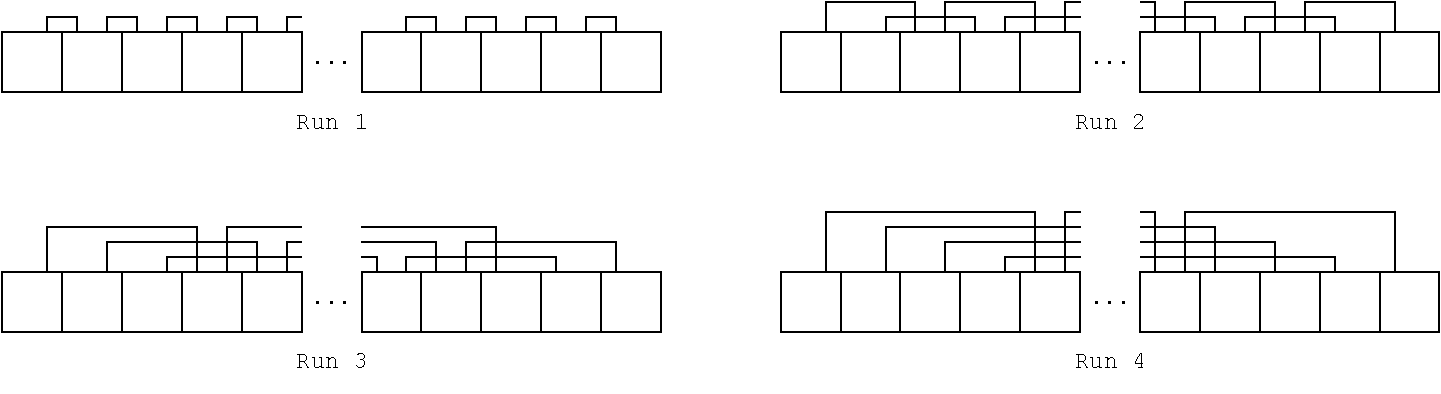
\includegraphics[width=\linewidth]{images/matrix-chain-order-ex.pdf}
    \caption{A diagram illustrating the upper and lower bound of the different sequences that $m(i, j)$ is calculated on for the first 4 runs.}
    \label{fig:matrix-chain-order-ex}
\end{figure}

\begin{remark}
    To get the parenthesization (instead of just the minimum number of multiplications needed) then we just construct another array $s$ for which we keep track of the paranthesization.
\end{remark}
